%\section{Design for Testability (DFT)}
\begin{frame}{Design for Testability (DFT)}
\begin{itemize}
\item Prevalently used to improve controllability/observability 
\item Industry DFT standard: Scan
\item Industry DFT Compression standard: Embedded Deterministic Test (EDT)
\end{itemize}
\end{frame}

\begin{frame}{Normal Circuit}
\begin{figure}
\begin{center}
\label{fig:scan-insertion}
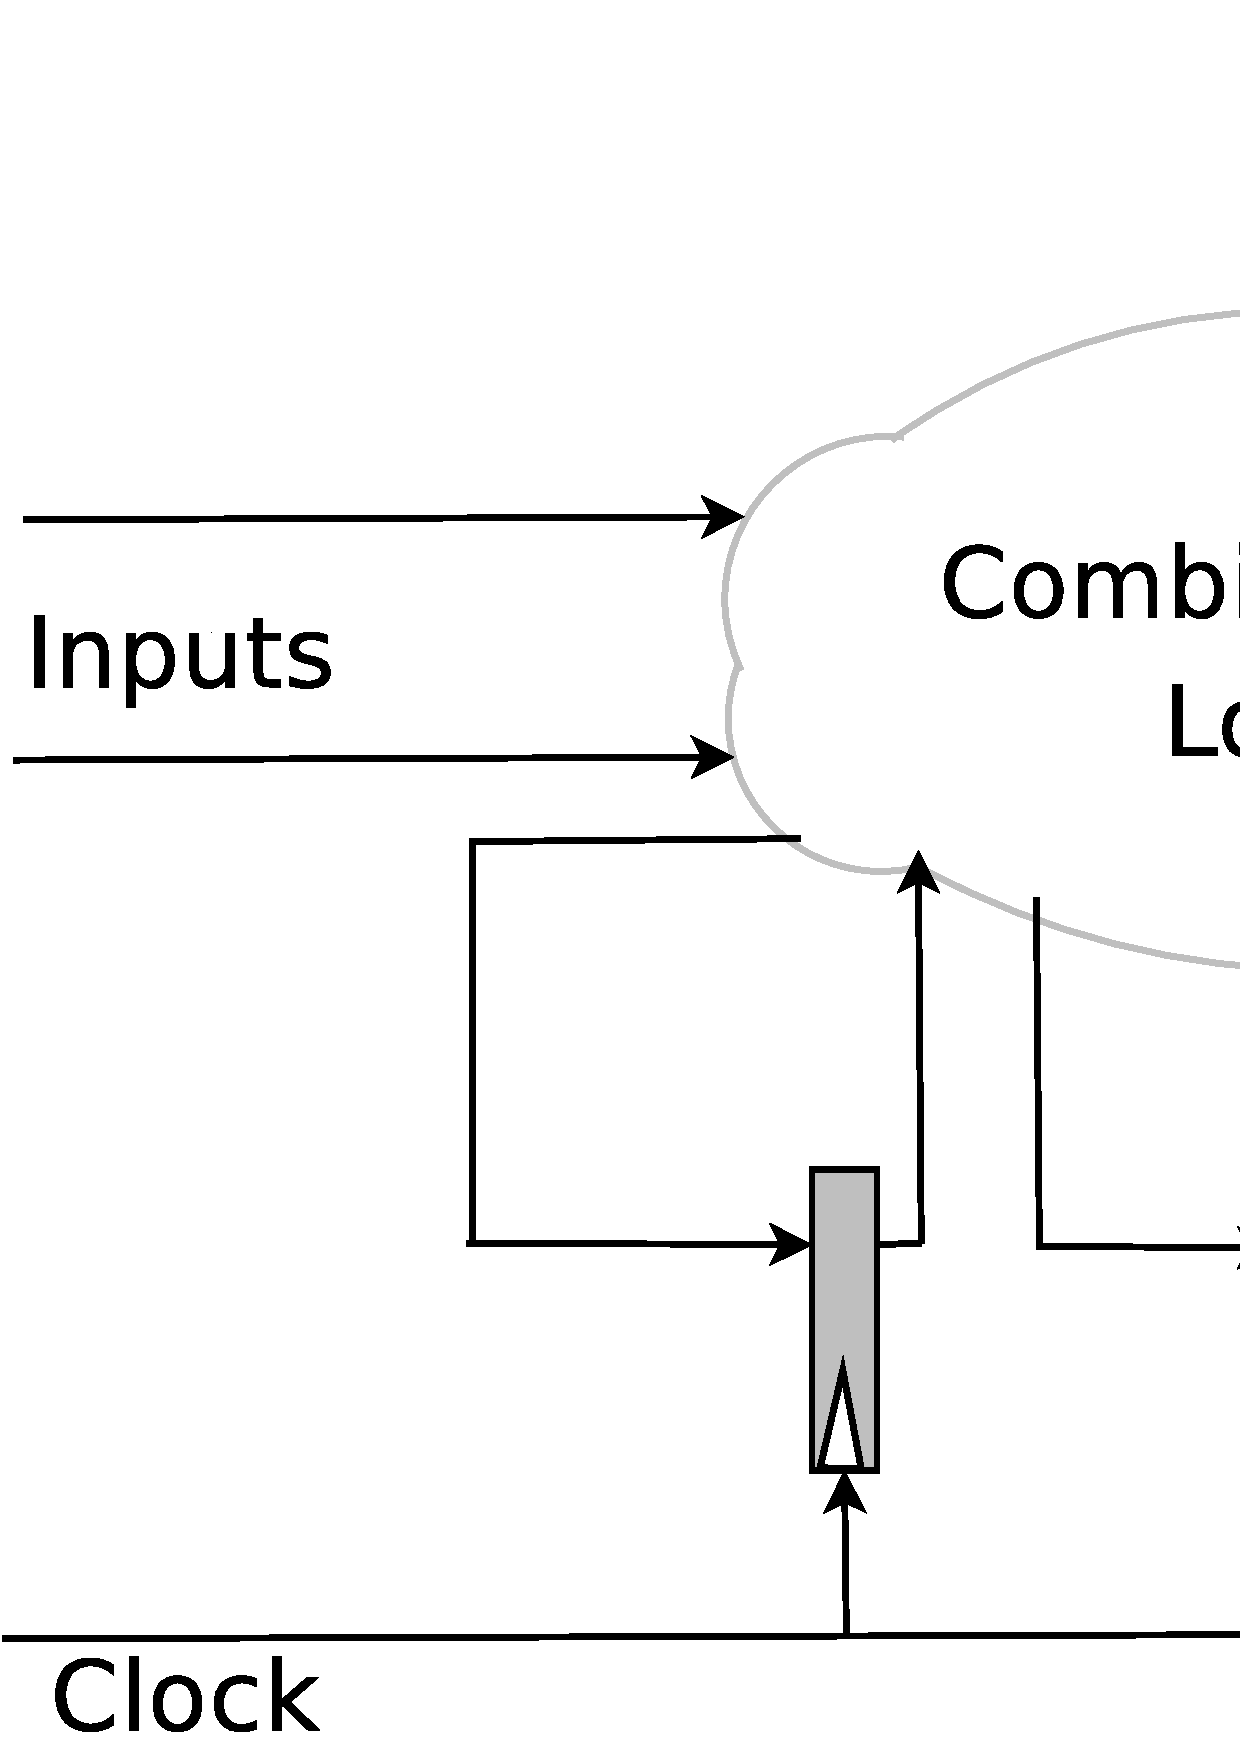
\includegraphics[scale=0.2]{fig/normal_circuit.pdf}
\end{center}
\end{figure}
\end{frame}

\begin{frame}{Circuit with Scan Insertion}

	\only<+>{
		\begin{figure}
		\begin{center}
		\label{fig:scan-insertion}
		\includegraphics[scale=0.2]{fig/scan_inserted_circuit.pdf}
		\end{center}
		\end{figure}
	}
	\only<+>{
		\begin{figure}		
		\begin{center}
		\caption{Shift mode}
		\label{fig:shift-mode}
		\includegraphics[scale=0.2]{fig/scan_inserted_circuit_shift_mode.pdf}
		\end{center}
		\end{figure}
	}
	\only<+>{
		\begin{figure}
		\begin{center}
		\caption{Capture mode}
		\label{fig:capture-mode}
		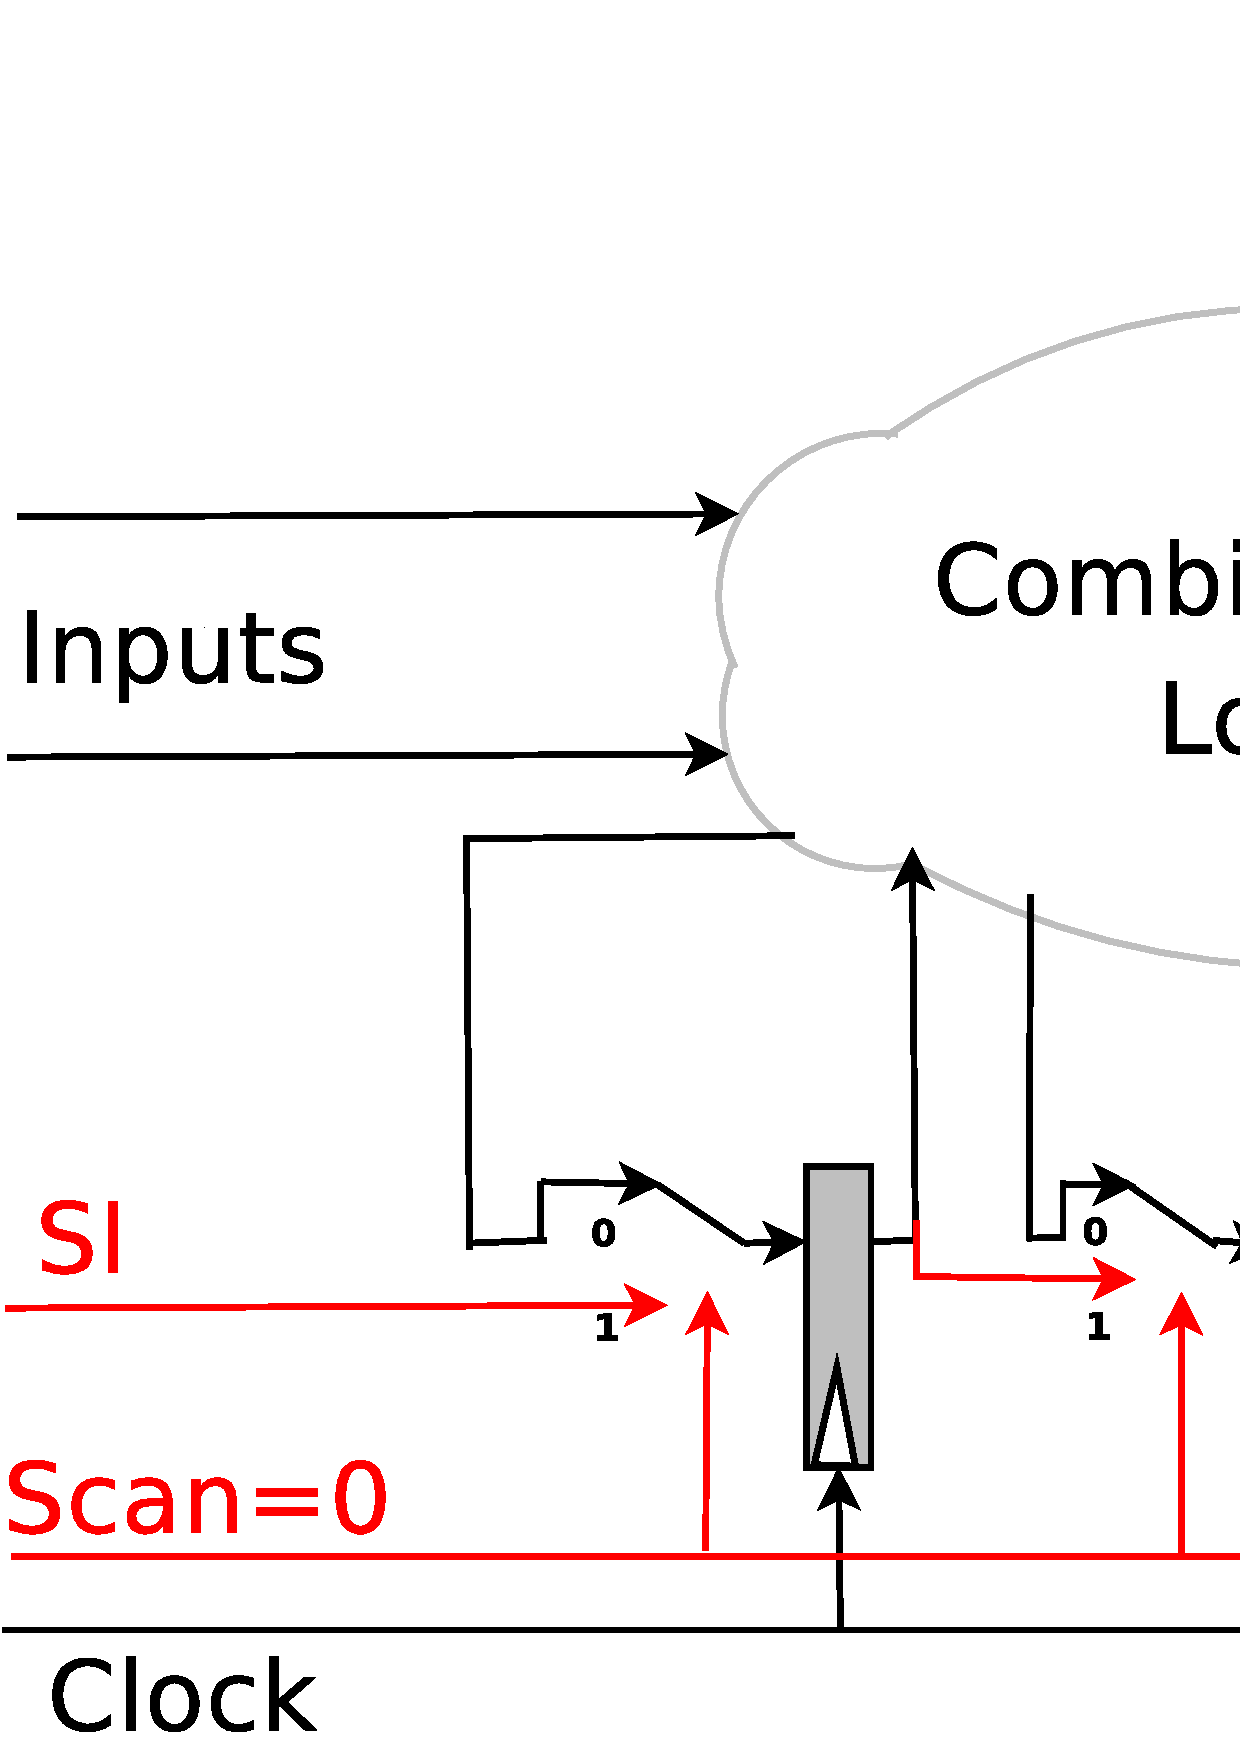
\includegraphics[scale=0.2]{fig/scan_inserted_circuit_capture_mode.pdf}
		\end{center}
		\end{figure}
	}
\end{frame}


\begin{frame}{Circuit with EDT Insertion}
\begin{figure}
\begin{center}
\label{fig:scan-mode}
\includegraphics[scale=0.2]{fig/EDT.pdf}
\end{center}
\end{figure}
\end{frame}


